\chapter{Theory}

In this chapter, I am going to describe the theories behind our experiment. It is divided into three parts. The first section explains the theories of cold Bose gas and the Bose-Einstein condensation relevant to the experiment. The second section briefly describes some important properties of the Lithium-$7$ atom. Finally, in the third section, the cooling, trapping and state manipulation techniques used in the experiment are presented, including Zeeman slower (\ref{theory:zeeman}), MOT(\ref{theory:mot}), gray molasses (\ref{theory:gm}), dark state pumping (\ref{theory:pump}), magnetic trap (\ref{theory:mt}) and optical dipole trap (\ref{theory:odt}).

\section{What is Bose-Einstein Condensate}\label{theory:bec}

Every real particles can be classified as one of the two families according to their spins, fermions which have half integer spins and bosons which have integer spins. According to quantum field theory\cite{spin-statistics1,spin-statistics2} the many-particles wave function of identical particles must be symmetric or anti-symmetric under particle exchange for bosons or fermions respectively. For bosonic particles, because of the symmetry of the wave function, the possibility for particles to be in the same state is greatly enhances. As a result, boson gas at ultra-low temperature forms a Bose-Einstein condensate (BEC), in which almost all of the particles are condensed to the lowest energy state. In the following, the relevant properties of BECs such as critical temperature and density distribution are described.

\subsection{BEC in Harmonic Trap}

Since the wave function of bosons is symmetric, multiple bosons can be in the same state. From this fact, the energy distribution can be calculated for bosons,
\eqar{
  f(\varepsilon)=&\frac{1}{\ue^{\beta(\varepsilon-\mu)} - 1}
}
Since the distribution has to be possitive for all energy states, in particular the $\varepsilon=0$ ground state, we have $\mu\geqslant0$. For all the state except the ground state, this sets an finite upper limit on the number of atoms in each state for a fixed temperature. Therefore, if the number of atoms exceeds a certain value, all the extra atoms will go into the ground state. These atoms condensed in the ground state are called the Bose Einstein condensate.\\
\\
In order to calculate the atom number in the condensate as well as the critical temperature, we can estimate the maximum atom number in the excited states (thermal atoms) with an integral,
\eqar{
  N_{th}=&\int_0^\infty\frac{g(\varepsilon)}{\ue^{\beta\varepsilon} - 1}\ud\varepsilon
}
where $g(\varepsilon)$ is the energy density of states. In our experiment, we create the BEC in a harmonic optical dipole trap (see \ref{theory:odt}) for which the energy density is,
\eqar{
  g(\varepsilon)=&\frac{\varepsilon^2}{2\hbar^3 \omega^3}\\
  N_{th}=&\frac{1}{2\hbar^3 \omega^3}\int_0^\infty\frac{\varepsilon^2}{\ue^{\beta\varepsilon} - 1}\ud\varepsilon\\
  =&\frac{1}{2\hbar^3 \omega^3\beta^3}\int_0^\infty\frac{x^2}{\ue^{x} - 1}\ud x\\
  =&\frac{k_B^3T^3}{2\hbar^3 \omega^3}\zeta(3)\Gamma(3)
}
The critical temperature of the transition, determined by $N_{th}=N$,
\eqar{
  T_C=&\frac{\hbar\omega}{k_B}\sqrt[3]{\frac{2N}{\zeta(3)\Gamma(3)}}\\
  =&0.9405\frac{\hbar\omega\sqrt[3]{N}}{k_B}
}
Condensate fraction (for large $N$),
\eqar{
  \frac{N_0}{N}=&1-\frac{N_{th}}{N}\\
  =&1-\paren{\frac{T}{T}}^3
}

\subsection{Effect of interaction}

The wavefunction of the condensed atoms is only the same with the single particle ground state wavefunction when there is no interaction between atoms. For interacting Bose gas this is no longer true. The

The ... only works for non-interacting.... when adding in interaction.... change shape..... this sub section describe .... in order to measure ....

\section{Lithium-$7$ Atoms}

The atoms used in this experiment is the Bosonic isotope of Lithium, Lithium-$7$. In this section, I will present some properties of the Lithium-$7$ atoms that are important for the cooling and traping techniques we use in the experiment.\\
\\
One of the most important properties for laser manipulation of cold atoms is the energy levels. As all other alkali atoms, Lithium-$7$ has one unpaired valence electron with a $nS$ ground state and $nP$ excited states, where $n=2$ for Lithium-$7$. The fine structure split the excited states into $2^2P_{1/2}$ and $2^2P_{3/2}$ states corresponding to the $D1$ and $D2$ lines that are about $10GHz$ apart. On top of these, the hyperfine structure caused by the nucleus spin ($I=3/2$ for Lithium-$7$) further split each of these states into different levels with different total angular momentum $F$. the precise frequencies of these transitions measured in the experiment are shown in figure \ref{li:lines}\\
\begin{figure}
  \begin{center}
    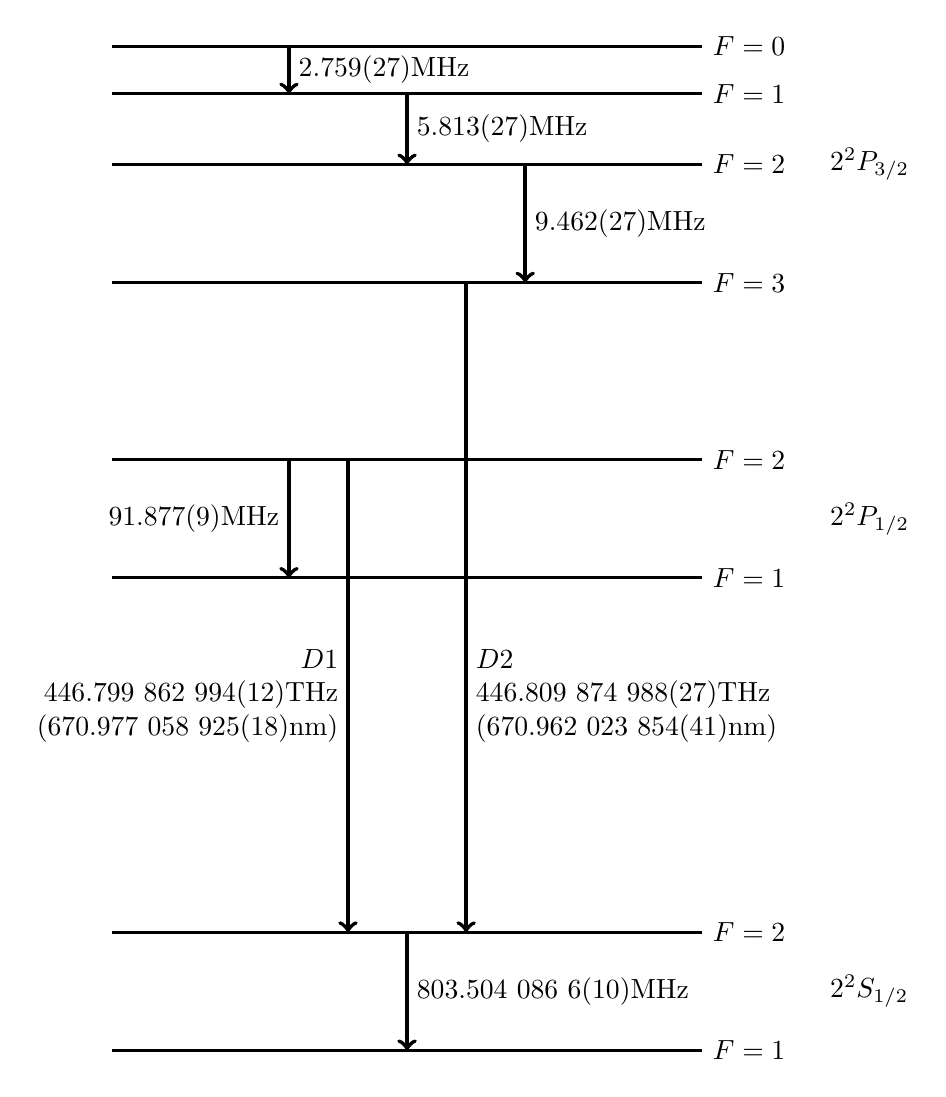
\begin{tikzpicture}[scale=1.5]
      % S1/2
      % F1
      \draw[line width=1] (0, 0) -- +(5, 0) node[right] {$F=1$};
      % F2
      \draw[line width=1] (0, 1) -- +(5, 0) node[right] {$F=2$};
      \path (6, 0.5) node[right] {$2^2S_{1/2}$};

      % P1/2
      % F1
      \draw[line width=1] (0, 4) -- +(5, 0) node[right] {$F=1$};
      % F2
      \draw[line width=1] (0, 5) -- +(5, 0) node[right] {$F=2$};
      \path (6, 4.5) node[right] {$2^2P_{1/2}$};

      % P3/2
      % F3
      \draw[line width=1] (0, 6.5) -- +(5, 0) node[right] {$F=3$};
      % F2
      \draw[line width=1] (0, 7.5) -- +(5, 0) node[right] {$F=2$};
      % F1
      \draw[line width=1] (0, 8.1) -- +(5, 0) node[right] {$F=1$};
      % F0
      \draw[line width=1] (0, 8.5) -- +(5, 0) node[right] {$F=0$};
      \path (6, 7.5) node[right] {$2^2P_{3/2}$};

      % D1
      \draw[line width=1.5,->] (2, 5) -- (2, 1);
      \path (2, 3) node[left,align=right] {$D1$\\$446.799\ 862\ 994(12)$THz\\ ($670.977\ 058\ 925(18)$nm)};

      % D2
      \draw[line width=1.5,->] (3, 6.5) -- (3, 1);
      \path (3, 3) node[right,align=left] {$D2$\\$446.809\ 874\ 988(27)$THz\\ ($670.962\ 023\ 854(41)$nm)};

      % S1/2
      \draw[line width=1.5,->] (2.5, 1) -- (2.5, 0);
      \path (2.5, .5) node[right] {$803.504\ 086\ 6(10)$MHz};

      % P1/2
      \draw[line width=1.5,->] (1.5, 5) -- (1.5, 4);
      \path (1.5, 4.5) node[left] {$91.877(9)$MHz};

      % P3/2
      \draw[line width=1.5,->] (3.5, 7.5) -- (3.5, 6.5);
      \path (3.5, 7) node[right] {$9.462(27)$MHz};
      \draw[line width=1.5,->] (2.5, 8.1) -- (2.5, 7.5);
      \path (2.5, 7.8) node[right] {$5.813(27)$MHz};
      \draw[line width=1.5,->] (1.5, 8.5) -- (1.5, 8.1);
      \path (1.5, 8.3) node[right] {$2.759(27)$MHz};
    \end{tikzpicture}
  \end{center}
  \caption{Energy levels of Lithium-$7$\cite{lithium-lines}}
  \label{li:lines}
\end{figure}\\
In an external magnetic field, each $F\neq0$ levels will be splited because of the Zeeman effect. At low field, this spliting is described by the Land\'e $g$-factor $\Delta=g_F\mu_Bm_FB_z$ as shown in table \ref{li7:g-factors}. At higher magnetic field, different hyperfine levels starts to mix and the Zeeman effect is nolonger linear. Most importantly, for $2^2S_{1/2}$ ground states the $F=1$ states have a negative slope at high magnetic field and all the $F=2$ states except $m_F=-2$ has a positive slope. (Note that $F$ and $m_F$ are nolonger good quantum numbers at high magnetic field but there are states at high field that are adabatically connected with these $F$ and $m_F$ eigenstates). The states with a positive Zeeman shift are called magnetically trappable states since they can be trapped by a static magnetic field with a minimum in the center. Only $|2, 2\rangle$ and $|2, 1\rangle$ are both trappable at high field and low field.

\begin{table}
  \caption{Land\'e $g$-factors of Lithium-$7$}
  \label{li7:g-factors}
  \begin{center}
    \begin{tabular}{|c|c|c|}\hline
      Fine Structure & $F$ & $g$-factor \\\hline
      $2^2S_{1/2}$ & $2$ & $\dfrac 12$ \\\cline{2-3}
      & $1$ & $-\dfrac 12$ \\\hline
      $2^2P_{1/2}$ & $2$ & $\dfrac 16$ \\\cline{2-3}
      & $1$ & $-\dfrac 16$ \\\hline
      $2^2P_{3/2}$ & $1$, $2$, $3$ & $\dfrac 23$ \\\hline
    \end{tabular}
  \end{center}
\end{table}

\section{Cooling and Traping Theory}

The atoms used in an alkali atom experiment often come from an atom beam coming out of a oven kept above the melting temperature of the metal. The oven used in this experiment operates at $485^\circ\text{C}$ producing an atom beam traveling at several hundred meters per second. In order to achieve low temperature and high density, several stages of slowing, traping and cooling are implemented in this experiment which finally bring the atoms down to the Bose-Einstein condensate condition. In this section, I am going to talk about the theory behind these techniques we are using in our experiment.

\subsection{Zeeman Slower}\label{theory:zeeman}

The atoms comes out of the oven has an average velocity determined by the Maxwell-Boltzmann distribution,
\eqar{
  \bar v=&\sqrt{\frac{k_BT}{2\pi m}}
}
We can slow down the atoms using the recoil of photon scattering by shining resonance light to the beam. However, since the atomic transition resonance is very narrow ($\Gamma=2\pi\cdot5.9\text{MHz}$) compare to the doppler shift ($\Delta\nu=\nu v/c\approx590\text{MHz}$), the atom will soon shift out of resonance once it slows down. There are several ways to solve this problem. One way is to modulate the laser frequency, either swiping with time (frequency chriping) or making it broadband (white light). The Zeeman slower solves the problem by changing the resonance of the atom with Zeeman effect. This is the most popular way for alkali atoms which usually have a cycling transition with linear Zeeman effect in a large range.\\
\\
The Zeeman slower has a magnetic field aligned with the atom beam with a spacially variant amplitude. By shining circularly polarized light against the atom beam, the atoms in the beam are optically pumped to one of the two stretch states determined by the relative direction of the field and the light polarization. If the magnetic field is changing in a way such that the Zeeman shift of the atom follows the Doppler shift when atoms slow down, the atom beam will be always in resonance and continuously being slowed down, i.e.
\eqar{
  g_Fm_F\mu_BB=\frac{v}{c}\nu+\Delta
}
For constant acceleration, this implies,
\eqar{
  B=\frac{\sqrt{v_0^2-2ax}}{g_Fm_F\mu_Bc}\nu+B_0
}
The maximum deceleration of the Zeeman slower is limited by the maximum scattering rate, therefore the life time of the excited state,
\eqar{
  a_{max}=&\frac{h\Gamma}{2\lambda}
}
where $\Gamma$ is the linewidth of the transition.

\subsection{Magneto-Optical Trap (MOT)}\label{theory:mot}

As in most cold atom experiment, our experiment starts with loading Zeeman slowed atom into a magneto-optical trap (MOT). MOT is a technique that uses laser and magnetic field gradient to provides both molasses cooling and confinement. In order to understand how MOT works, we will consider a one-dimensional model consisting of a spacially varying magnetic field $B=B_x=B'x$, two counter propagating, red-detuned, circularly polarized light with atoms sitting close to the zero of the magnetic field.\\
\\
The cooling and traping effect in a MOT can be understood separately. Let us first consider an atom in the center of the MOT moving in the $+x$ direction. Since the light is red-detuned, the Doppler effect will shift the atom closer to the light in $-x$ direction and farther from the light in $+x$ direction. The atom will therefore scatters more photons from the $-x$ light and experience an average force proportional but in the opposite direction with its velocity. Such a force will damp the motion of the atom and therefore cool down the temperature of the cloud.\\
\\
In order to understand the source of the traping force in a MOT, we can consider an atom with a $F=0$ ground state and $F=1$ excited states. As we can see in the schematic of this model (Figure \ref{mot:energy}), since the magnetic field changes its direction in the center, both laser beams are $\sigma^-$ light on the side it is coming from and therefore is shifted closer to resonance by the Zeeman effect. Therefore, atoms shifted from the center will scatter more photon from this direction and on average feel a net force from recoil pointing toward the center of the trap.\\
\begin{figure}
  \begin{center}
    \begin{tikzpicture}[scale=2]
      % axis
      \draw[line width=1.3,->] (-2.5, 0) -- (2.5, 0) node[below] {$x$};
      \draw[line width=1.3,->] (0, 0) -- (0, 3.5) node[right] {$\omega$};

      % Zeeman levels
      % F = 1
      \draw[line width=1] (-1.5, 2.5) -- (1.5, 2.5);
      \draw[line width=1] (-1.5, 3) -- (1.5, 2);
      \draw[line width=1] (-1.5, 2) -- (1.5, 3);

      % F = 0
      \draw[line width=1] (-1.5, .2) -- (1.5, .2);

      % Light freq
      \draw[line width=1,dashed] (-1.5, 1.8) -- (1.5, 1.8) node[below right] {Laser Frequency};

      % Zeeman labels
      \path (1.5, 3.5) node[right] {$|F, m_F\rangle$};
      \path (1.5, 3) node[right] {$|1, 1\rangle$};
      \path (1.5, 2.5) node[right] {$|1, 0\rangle$};
      \path (1.5, 2) node[right] {$|1, -1\rangle$};
      \path (1.5, .2) node[right] {$|0, 0\rangle$};

      \path (-1.5, 3.5) node[left] {$|F, m_F\rangle$};
      \path (-1.5, 3) node[left] {$|1, 1\rangle$};
      \path (-1.5, 2.5) node[left] {$|1, 0\rangle$};
      \path (-1.5, 2) node[left] {$|1, -1\rangle$};
      \path (-1.5, .2) node[left] {$|0, 0\rangle$};

      % Light polarization
      \draw[line width=1,snake arrow] (-1.5, 1.2) node[left] {$+x$ polarization} -- (1.5, 1.2);
      \draw[line width=2,->] (-1.2, 1.2) [partial ellipse=30:330:0.1 and 0.2];
      \path (-0.7, 1.2) node[above] {$\sigma^-$};
      \path (0.7, 1.2) node[above] {$\sigma^+$};

      \draw[line width=1,snake arrow] (1.5, 0.7) node[right] {$-x$ polarization} -- (-1.5, 0.7);
      \draw[line width=2,->] (1.2, 0.7) [partial ellipse=330:30:0.1 and 0.2];
      \path (0.7, 0.7) node[below] {$\sigma^-$};
      \path (-0.7, 0.7) node[below] {$\sigma^+$};

    \end{tikzpicture}
  \end{center}
  \caption{Schematic of a $1D$ MOT with a $F = 0$ to $F = 1$ transition.}
  \label{mot:energy}
\end{figure}\\
The performance of the MOT is usually limited by the random kick from scattered photons (Doppler limit on temperature) and light induced collisions (limits the density and atom number).

\subsection{Gray Molasses}\label{theory:gm}

Since the $2^2P_{3/2}$ excited state of Lithium-$7$ we use for molasses cooling in the MOT does not have resolved hyperfine structure (Figure \ref{li:lines}). We cannot preform conventional polarization gradient cooling using the $D2$ line. Instead, we implement a gray molasses on the D1 transition. This scheme was first studied and demonstrated by Christophe Salomon\cite{gm-theory} to achieve sub-Doppler temperature on some alkali isotopes that are not amenable for conventional polarization cooling ($^7Li$, $^6Li$ and $^{40}K$). In this section, I am going to present a semi-quantitative explanation of this cooling scheme. See the original paper\cite{gm-theory} for more detail discussion.\\
\\
The gray molasses cooling uses three pairs of counter-propagating beams that can cool the cloud in all three dimensions. Like what we did for MOT, we will consider a $1-D$ case for simplicity. The model we will use has a pair of counter-propagating beams, each has a high intensity pumper, with a large blue detuning $\delta$ from the $F=2$ ($|2\rangle$) to $F'=2$ ($|3\rangle$) $D1$ transition, and a low intensity repumper, blue detuned from the $F=1$ ($|1\rangle$) to $F'=2$ $D1$ transition by the same detuning $\delta$. Let the Rabi frequency for the pumper and the repumper be $\Omega_2(x)$ and $\Omega_1(x)$ respectively.\\
\\
Just as any other laser cooling method, the performance of the gray molasses is determined by the balance between cooling force and heating from photon scattering. Since the two beams (pumper and repumper) satisfies the Raman resonance condition, the system has a dark state which is the superposition of $|1\rangle$ and $|2\rangle$,
\eqar{
  |NC\rangle=&\frac{\Omega_2|1\rangle-\Omega_1|2\rangle}{\sqrt{\Omega_1^2+\Omega_2^2}}
}
which will be the state most of the atoms will be pumped into. (The state is dark for stationary atoms and has a non-zero but small scattering rate for moving atoms.) Since the scattering is suppressed by the present of a dark state, the gray molasses produce little heating.\\
\begin{figure}
  \begin{center}
    \begin{tikzpicture}
      % axis
      \draw[line width=1.3,->] (-2, 0) -- (5, 0) node[below] {$x$};
      \draw[line width=1.3,->] (-2, 0) -- ++(0, 8) node[above] {$E$};

      % Dressed levels 1
      \draw[line width=2] plot[id=x,domain=1:4,samples=1000] function{3 + 0.2 * sin(5 * x)} node[right] {$|3',n-1\rangle$};
      \draw[line width=1] plot[id=x,domain=1:4,samples=1000] function{4.2 - 0.2 * sin(5 * x)};
      \draw[line width=1] plot[id=x,domain=1:4,samples=1000] function{4.215 - 0.215 * sin(5 * x)} node[right] {$|2',n\rangle$};
      \draw[line width=1] plot[id=x,domain=1:4,samples=1000] function{4.23 - 0.23 * sin(5 * x)};
      \draw[dashed] (1, 3.986) -- ++(3, 0);

      % Dressed levels 2
      \draw[line width=2] plot[id=x,domain=1:4,samples=1000] function{6.5 + 0.2 * sin(5 * x)} node[right] {$|3',n\rangle$};
      \draw[line width=1] plot[id=x,domain=1:4,samples=1000] function{7.7 - 0.2 * sin(5 * x)} node[right] {$|2',n+1\rangle$};
      \draw[line width=1] plot[id=x,domain=1:4,samples=1000] function{7.715 - 0.215 * sin(5 * x)};
      \draw[line width=1] plot[id=x,domain=1:4,samples=1000] function{7.73 - 0.23 * sin(5 * x)};
      \draw[dashed] (1, 7.486) -- ++(3, 0);

      % F1 states
      \draw (0.5, 0.5) -- ++(-0.5, 0) node[left] {$|1,n-1\rangle$};
      \draw (0.5, 3.5) -- ++(-0.5, 0) node[left] {$|1,n\rangle$};

      % Repumper
      \draw[red,line width=1,dashed] (pi / 2 - 0.25, 7.35) -- ++(0.5, 0);
      \draw[red,line width=1,snake arrow] (0.25, 3.5) -- (pi / 2, 7.35);
      \draw[red,line width=1,snake arrow] (pi / 2, 7.35) -- (pi / 2, 4);
      \draw[red,line width=2.6] plot[id=x,domain=pi / 2:(pi * 0.7 + 0.1),samples=1000] function{4.215 - 0.215 * sin(5 * x)};
      % Somehow math functions does not work correctly here.
      \draw[red,line width=1,snake arrow] (pi * 0.7 + 0.1, 4.215 + 0.215 * 0.87758256189037287) -- (0.25, 0.5);
    \end{tikzpicture}
  \end{center}
  \caption{Schematic of a $1D$ Gray Molasses.\cite{gm-theory}}
  \label{gm:dressed}
\end{figure}\\
The cooling effect of the gray molasses can be understood in the dressed atom picture for the atom and the pumper beam as shown in figure \ref{gm:dressed}, where,
\eqar{
  |2'\rangle=&\frac{\delta^2}{\delta^2+\Omega_2(x)^2}\paren{|2\rangle-\ui\Omega_2(x)|3\rangle}\\
  |3'\rangle=&\frac{\delta^2}{\delta^2+\Omega_2(x)^2}\paren{|3\rangle-\ui\Omega_2(x)|2\rangle}
}
Since the detuning $\delta$ is large, the mixing between $|2\rangle$ and $|3\rangle$ is small leaving $|3'\rangle$ a short lifetime and $|2'\rangle$ a longer lifetime. The two counter-propagating pumper beams create a standing wave which causes periodic AC-Stark shift in the dressed $|2'\rangle$ and $|3'\rangle$ states. For a repumper with the same or slightly smaller blue detuning compare to the pumper. It is the most closest to the resonance with the dressed states at the nodes of the standing wave where the mixing is minimized. Therefore, the repumper will most likely pumps atoms into the $|2'\rangle$ state (through $|3'\rangle$ as shown in figure \ref{gm:dressed}) at the node of the standing wave and the atoms will most likely exit the state at the anti-node of the standing wave where the lifetime of $|2'\rangle$ is the shortest because of the maximum mixing. Since potential enery for atoms in $|2'\rangle$ is minimized at the nodes and maximized at the anti-nodes the atoms will on average feel a damping force by climbing up the hill in $|2'\rangle$. The height of the hill, therefore the cooling force, is proportional to the laser intensity. Combined with the low scattering rate due to the dark state, the gray molasses can be used to quickly cool the cloud after MOT to sub-Doppler temperature.

\subsection{Dark State Pumping}\label{theory:pump}

At the end of Laser cooling, the atoms are distributed in different ground states.\\
In order to trap in MT, need to go to 2, 2 / 2, 1 which are the only trappable states at both low field and high field.\\
Choose 2, 2 because we can use dark state pumping which ...

Dark State pumping with D1 light

\subsection{Evaporation in Static Magnetic Trap}\label{theory:mt}
Trapable states
Power law?

\subsection{Evaporation in Optical Dipole Trap}\label{theory:odt}
AC Stark Shift
Cross ODT
Feshbach resonance
